\documentclass[11pt,fleqn]{book}

\def\ldp{(\!\!(} 
\def\rdp{)\!\!)}

\def\corrige{1}
\usepackage{amsmath}
\usepackage{mathtools}
\usepackage[french]{babel}
\selectlanguage{french}
\usepackage[utf8]{inputenc}
\newcommand{\graphe}[2]{\includegraphics[width=#1]{#2}}%
\newcommand{\tabref}[1]{Tab.~\ref{#1}}
\newcommand{\figref}[1]{Fig.~\ref{#1}}
\newcommand{\defref}[1]{Def.~\ref{#1}}
\newcommand{\chapref}[1]{Chap.~\ref{#1}}
\newcommand{\secref}[1]{\S\ref{#1}}
\def\cad{c.-à-d.}

\newcommand{\imagetexte}[4]{\begin{minipage}{#1\linewidth}
\graphe{\linewidth}{#2}
\end{minipage}\hfill
\begin{minipage}{#3\linewidth}
#4
\end{minipage}}

\newcommand{\texteimage}[4]{\begin{minipage}{#3\linewidth}
#4
\end{minipage}\hfill
\begin{minipage}{#1\linewidth}
\graphe{\linewidth}{#2}
\end{minipage}}

\newcommand{\refjupyter}[1]{Notebook\ref{#1}} % les defs du style du poly
%%%%%%%%%%%%%%%%%%%%%%%%%%%%%%%%%%%%%%%%%
% The Legrand Orange Book
% Structural Definitions File
% Version 2.1 (26/09/2018)
%
% Original author:
% Mathias Legrand (legrand.mathias@gmail.com) with modifications by:
% Vel (vel@latextemplates.com)
% 
% This file was downloaded from:
% http://www.LaTeXTemplates.com
%
% License:
% CC BY-NC-SA 3.0 (http://creativecommons.org/licenses/by-nc-sa/3.0/)
%
%%%%%%%%%%%%%%%%%%%%%%%%%%%%%%%%%%%%%%%%%

%----------------------------------------------------------------------------------------
%	VARIOUS REQUIRED PACKAGES AND CONFIGURATIONS
%----------------------------------------------------------------------------------------

\usepackage{graphicx} % Required for including pictures
\graphicspath{{./tikz/}{./dessins/}{./Pictures/}} % Specifies the directory where pictures are stored

\usepackage{lipsum} % Inserts dummy text

\usepackage{tikz} % Required for drawing custom shapes


\usepackage{enumitem} % Customize lists
\setlist{nolistsep} % Reduce spacing between bullet points and numbered lists

\usepackage{booktabs} % Required for nicer horizontal rules in tables
\usepackage{tabularx} % Required for nicer horizontal rules in tables
\usepackage{lscape}
\usepackage{xcolor} % Required for specifying colors by name
\definecolor{ocre}{RGB}{243,102,25} % Define the orange color used for highlighting throughout the book
\definecolor{vert}{RGB}{102,243,25} % Define the orange color used for highlighting throughout the book

%----------------------------------------------------------------------------------------
%	MARGINS
%----------------------------------------------------------------------------------------

\usepackage{geometry} % Required for adjusting page dimensions and margins

\geometry{
	paper=a4paper, % Paper size, change to letterpaper for US letter size
	top=3cm, % Top margin
	bottom=3cm, % Bottom margin
	left=3cm, % Left margin
	right=3cm, % Right margin
	headheight=14pt, % Header height
	footskip=1.4cm, % Space from the bottom margin to the baseline of the footer
	headsep=10pt, % Space from the top margin to the baseline of the header
	%showframe, % Uncomment to show how the type block is set on the page
}

%----------------------------------------------------------------------------------------
%	FONTS
%----------------------------------------------------------------------------------------

\usepackage{avant} % Use the Avantgarde font for headings
%\usepackage{times} % Use the Times font for headings
\usepackage{mathptmx} % Use the Adobe Times Roman as the default text font together with math symbols from the Sym­bol, Chancery and Com­puter Modern fonts

\usepackage{microtype} % Slightly tweak font spacing for aesthetics

%----------------------------------------------------------------------------------------
%	BIBLIOGRAPHY AND INDEX
%----------------------------------------------------------------------------------------
\usepackage{csquotes}
%\usepackage[style=numeric,citestyle=numeric,sorting=nyt,sortcites=true,autopunct=true,autolang=hyphen,hyperref=true,abbreviate=false,backref=true,backend=biber]{biblatex}
%\addbibresource{bibliography.bib} % BibTeX bibliography file
%\defbibheading{bibempty}{}

\usepackage{calc} % For simpler calculation - used for spacing the index letter headings correctly
\usepackage{makeidx} % Required to make an index
\makeindex % Tells LaTeX to create the files required for indexing

%----------------------------------------------------------------------------------------
%	MAIN TABLE OF CONTENTS
%----------------------------------------------------------------------------------------

\usepackage{titletoc} % Required for manipulating the table of contents

\contentsmargin{0cm} % Removes the default margin

% Part text styling (this is mostly taken care of in the PART HEADINGS section of this file)
\titlecontents{part}
	[0cm] % Left indentation
	{\addvspace{20pt}\bfseries} % Spacing and font options for parts
	{}
	{}
	{}

% Chapter text styling
\titlecontents{chapter}
	[1.25cm] % Left indentation
	{\addvspace{12pt}\large\sffamily\bfseries} % Spacing and font options for chapters
	{\color{ocre!60}\contentslabel[\Large\thecontentslabel]{1.25cm}\color{ocre}} % Formatting of numbered sections of this type
	{\color{ocre}} % Formatting of numberless sections of this type
	{\color{ocre!60}\normalsize\;\titlerule*[.5pc]{.}\;\thecontentspage} % Formatting of the filler to the right of the heading and the page number

% Section text styling
\titlecontents{section}
	[1.25cm] % Left indentation
	{\addvspace{3pt}\sffamily\bfseries} % Spacing and font options for sections
	{\contentslabel[\thecontentslabel]{1.25cm}} % Formatting of numbered sections of this type
	{} % Formatting of numberless sections of this type
	{\hfill\color{black}\thecontentspage} % Formatting of the filler to the right of the heading and the page number

% Subsection text styling
\titlecontents{subsection}
	[1.25cm] % Left indentation
	{\addvspace{1pt}\sffamily\small} % Spacing and font options for subsections
	{\contentslabel[\thecontentslabel]{1.25cm}} % Formatting of numbered sections of this type
	{} % Formatting of numberless sections of this type
	{\ \titlerule*[.5pc]{.}\;\thecontentspage} % Formatting of the filler to the right of the heading and the page number

% Figure text styling
\titlecontents{figure}
	[1.25cm] % Left indentation
	{\addvspace{1pt}\sffamily\small} % Spacing and font options for figures
	{\thecontentslabel\hspace*{1em}} % Formatting of numbered sections of this type
	{} % Formatting of numberless sections of this type
	{\ \titlerule*[.5pc]{.}\;\thecontentspage} % Formatting of the filler to the right of the heading and the page number

% Table text styling
\titlecontents{table}
	[1.25cm] % Left indentation
	{\addvspace{1pt}\sffamily\small} % Spacing and font options for tables
	{\thecontentslabel\hspace*{1em}} % Formatting of numbered sections of this type
	{} % Formatting of numberless sections of this type
	{\ \titlerule*[.5pc]{.}\;\thecontentspage} % Formatting of the filler to the right of the heading and the page number

%----------------------------------------------------------------------------------------
%	MINI TABLE OF CONTENTS IN PART HEADS
%----------------------------------------------------------------------------------------

% Chapter text styling
\titlecontents{lchapter}
	[0em] % Left indentation
	{\addvspace{15pt}\large\sffamily\bfseries} % Spacing and font options for chapters
	{\color{ocre}\contentslabel[\Large\thecontentslabel]{1.25cm}\color{ocre}} % Chapter number
	{}  
	{\color{ocre}\normalsize\sffamily\bfseries\;\titlerule*[.5pc]{.}\;\thecontentspage} % Page number

% Section text styling
\titlecontents{lsection}
	[0em] % Left indentation
	{\sffamily\small} % Spacing and font options for sections
	{\contentslabel[\thecontentslabel]{1.25cm}} % Section number
	{}
	{}

% Subsection text styling (note these aren't shown by default, display them by searchings this file for tocdepth and reading the commented text)
\titlecontents{lsubsection}
	[.5em] % Left indentation
	{\sffamily\footnotesize} % Spacing and font options for subsections
	{\contentslabel[\thecontentslabel]{1.25cm}}
	{}
	{}

%----------------------------------------------------------------------------------------
%	HEADERS AND FOOTERS
%----------------------------------------------------------------------------------------

\usepackage{fancyhdr} % Required for header and footer configuration

\pagestyle{fancy} % Enable the custom headers and footers

\renewcommand{\chaptermark}[1]{\markboth{\sffamily\normalsize\bfseries\chaptername\ \thechapter.\ #1}{}} % Styling for the current chapter in the header
\renewcommand{\sectionmark}[1]{\markright{\sffamily\normalsize\thesection\hspace{5pt}#1}{}} % Styling for the current section in the header

\fancyhf{} % Clear default headers and footers
\fancyhead[LE,RO]{\sffamily\normalsize\thepage} % Styling for the page number in the header
\fancyhead[LO]{\rightmark} % Print the nearest section name on the left side of odd pages
\fancyhead[RE]{\leftmark} % Print the current chapter name on the right side of even pages
%\fancyfoot[C]{\thepage} % Uncomment to include a footer

\renewcommand{\headrulewidth}{0.5pt} % Thickness of the rule under the header

\fancypagestyle{plain}{% Style for when a plain pagestyle is specified
	\fancyhead{}\renewcommand{\headrulewidth}{0pt}%
}

% Removes the header from odd empty pages at the end of chapters
\makeatletter
\renewcommand{\cleardoublepage}{
\clearpage\ifodd\c@page\else
\hbox{}
\vspace*{\fill}
\thispagestyle{empty}
\newpage
\fi}

%----------------------------------------------------------------------------------------
%	THEOREM STYLES
%----------------------------------------------------------------------------------------

\usepackage{amsmath,amsfonts,amssymb,amsthm} % For math equations, theorems, symbols, etc

\newcommand{\intoo}[2]{\mathopen{]}#1\,;#2\mathclose{[}}
\newcommand{\ud}{\mathop{\mathrm{{}d}}\mathopen{}}
\newcommand{\intff}[2]{\mathopen{[}#1\,;#2\mathclose{]}}
\renewcommand{\qedsymbol}{$\blacksquare$}
\newtheorem{notation}{Notation}[chapter]

% Boxed/framed environments
\newtheoremstyle{ocrenumbox}% Theorem style name
{0pt}% Space above
{0pt}% Space below
{\normalfont}% Body font
{}% Indent amount
{\small\bf\sffamily\color{ocre}}% Theorem head font
{\;}% Punctuation after theorem head
{0.25em}% Space after theorem head
{\small\sffamily\color{ocre}\thmname{#1}\nobreakspace\thmnumber{\@ifnotempty{#1}{}\@upn{#2}}% Theorem text (e.g. Theorem 2.1)
\thmnote{\nobreakspace\the\thm@notefont\sffamily\bfseries\color{black}---\nobreakspace#3.}} % Optional theorem note

\newtheoremstyle{blacknumex}% Theorem style name
{5pt}% Space above
{5pt}% Space below
{\normalfont}% Body font
{} % Indent amount
{\small\bf\sffamily}% Theorem head font
{\;}% Punctuation after theorem head
{0.25em}% Space after theorem head
{\small\sffamily{\tiny\ensuremath{\blacksquare}}\nobreakspace\thmname{#1}\nobreakspace\thmnumber{\@ifnotempty{#1}{}\@upn{#2}}% Theorem text (e.g. Theorem 2.1)
\thmnote{\nobreakspace\the\thm@notefont\sffamily\bfseries---\nobreakspace#3.}}% Optional theorem note

\newtheoremstyle{blacknumbox} % Theorem style name
{0pt}% Space above
{0pt}% Space below
{\normalfont}% Body font
{}% Indent amount
{\small\bf\sffamily}% Theorem head font
{\;}% Punctuation after theorem head
{0.25em}% Space after theorem head
{\small\sffamily\thmname{#1}\nobreakspace\thmnumber{\@ifnotempty{#1}{}\@upn{#2}}% Theorem text (e.g. Theorem 2.1)
\thmnote{\nobreakspace\the\thm@notefont\sffamily\bfseries---\nobreakspace#3.}}% Optional theorem note

% Non-boxed/non-framed environments
\newtheoremstyle{ocrenum}% Theorem style name
{5pt}% Space above
{5pt}% Space below
{\normalfont}% Body font
{}% Indent amount
{\small\bf\sffamily\color{ocre}}% Theorem head font
{\;}% Punctuation after theorem head
{0.25em}% Space after theorem head
{\small\sffamily\color{ocre}\thmname{#1}\nobreakspace\thmnumber{\@ifnotempty{#1}{}\@upn{#2}}% Theorem text (e.g. Theorem 2.1)
\thmnote{\nobreakspace\the\thm@notefont\sffamily\bfseries\color{black}---\nobreakspace#3.}} % Optional theorem note
\makeatother

% Defines the theorem text style for each type of theorem to one of the three styles above
\newcounter{dummy} 
\numberwithin{dummy}{section}
\theoremstyle{ocrenumbox}
\newtheorem{theoremeT}[dummy]{Theorème}
\newtheorem{demoT}[]{Démonstration}
\newtheorem{probleme}{Problème}[chapter]
\newtheorem{exerciseT}{Exercice}[chapter]
\theoremstyle{blacknumex}
\newtheorem{exempleT}{Exemple}[chapter]
\newtheorem{competencesT}{Compétences}[]
\theoremstyle{blacknumbox}
\newtheorem{vocabulary}{Vocabulary}[chapter]
\newtheorem{definitionT}{Definition}[section]
\newtheorem{corollaryT}[dummy]{Corollary}
\theoremstyle{ocrenum}
\newtheorem{proposition}[dummy]{Proposition}

%----------------------------------------------------------------------------------------
%	DEFINITION OF COLORED BOXES
%----------------------------------------------------------------------------------------

\RequirePackage[framemethod=default]{mdframed} % Required for creating the theorem, definition, exercislse and corollary boxes

% Theorem box
\newmdenv[skipabove=7pt,
skipbelow=7pt,
backgroundcolor=black!5,
linecolor=ocre,
innerleftmargin=5pt,
innerrightmargin=5pt,
innertopmargin=5pt,
leftmargin=0cm,
rightmargin=0cm,
innerbottommargin=5pt]{tBox}

% Exercise box	  
\newmdenv[skipabove=7pt,
skipbelow=7pt,
rightline=false,
leftline=true,
topline=false,
bottomline=false,
backgroundcolor=ocre!10,
linecolor=ocre,
innerleftmargin=5pt,
innerrightmargin=5pt,
innertopmargin=5pt,
innerbottommargin=5pt,
leftmargin=0cm,
rightmargin=0cm,
linewidth=4pt]{eBox}	

% Definition box
\newmdenv[skipabove=7pt,
skipbelow=7pt,
rightline=false,
leftline=true,
topline=false,
bottomline=false,
linecolor=ocre,
innerleftmargin=5pt,
innerrightmargin=5pt,
innertopmargin=0pt,
leftmargin=0cm,
rightmargin=0cm,
linewidth=4pt,
innerbottommargin=0pt]{dBox}	

% Corollary box
\newmdenv[skipabove=7pt,
skipbelow=7pt,
rightline=false,
leftline=true,
topline=false,
bottomline=false,
linecolor=gray,
backgroundcolor=black!5,
innerleftmargin=5pt,
innerrightmargin=5pt,
innertopmargin=5pt,
leftmargin=0cm,
rightmargin=0cm,
linewidth=4pt,
innerbottommargin=5pt]{cBox}

% Creates an environment for each type of theorem and assigns it a theorem text style from the "Theorem Styles" section above and a colored box from above
\newenvironment{theoreme}{\begin{tBox}\begin{theoremeT}}{\end{theoremeT}\end{tBox}}
\newenvironment{demo}{\begin{cBox}\begin{demoT}}{\hfill{\color{ocre}\tiny\ensuremath{\blacksquare}}\end{demoT}\end{cBox}}			
\newenvironment{exercise}{\begin{eBox}\begin{exerciseT}}{\hfill{\color{ocre}\tiny\ensuremath{\blacksquare}}\end{exerciseT}\end{eBox}}				  
\newenvironment{definition}{\begin{eBox}\begin{definitionT}}{\end{definitionT}\end{eBox}}	
\newenvironment{exemple}{\begin{exempleT}}{\hfill{\tiny\ensuremath{\blacksquare}}\end{exempleT}}		
\newenvironment{corollary}{\begin{cBox}\begin{corollaryT}}{\end{corollaryT}\end{cBox}}	
\newenvironment{competences}{\begin{eBox}\begin{competencesT}}{\end{competencesT}\end{eBox}}	


%----------------------------------------------------------------------------------------
%   ENVIRONMENT POUR MOI
%----------------------------------------------------------------------------------------

\newenvironment{exercice}{\begin{eBox}\begin{exerciseT}}{\hfill{\color{ocre}\tiny\ensuremath{\blacksquare}}\end{exerciseT}\end{eBox}}				  

\def\remarqueTitre#1{\textcolor{ocre}{\textbf{#1}}\\}
\def\exerciceTitre#1{\textcolor{ocre}{\textbf{#1}}\\}

\newenvironment{quizz}{\begin{eBox} QUIZZ}{\hfill{\color{vert}}\end{eBox}}				  
\newenvironment{citations}{\begin{cBox}}{\end{cBox}}	


%----------------------------------------------------------------------------------------
%	REMARK ENVIRONMENT
%----------------------------------------------------------------------------------------

\newenvironment{remarque}{\par\vspace{10pt}\small % Vertical white space above the remark and smaller font size
\begin{list}{}{
\leftmargin=35pt % Indentation on the left
\rightmargin=25pt}\item\ignorespaces % Indentation on the right
\makebox[-2.5pt]{\begin{tikzpicture}[overlay]
\node[draw=ocre!60,line width=1pt,circle,fill=ocre!25,font=\sffamily\bfseries,inner sep=2pt,outer sep=0pt] at (-15pt,0pt){\textcolor{ocre}{R}};\end{tikzpicture}} % Orange R in a circle
\advance\baselineskip -1pt}{\end{list}\vskip5pt} % Tighter line spacing and white space after remark

%----------------------------------------------------------------------------------------
%	SECTION NUMBERING IN THE MARGIN
%----------------------------------------------------------------------------------------

\makeatletter
\renewcommand{\@seccntformat}[1]{\llap{\textcolor{ocre}{\csname the#1\endcsname}\hspace{1em}}}                    
\renewcommand{\section}{\@startsection{section}{1}{\z@}
{-4ex \@plus -1ex \@minus -.4ex}
{1ex \@plus.2ex }
{\normalfont\large\sffamily\bfseries}}
\renewcommand{\subsection}{\@startsection {subsection}{2}{\z@}
{-3ex \@plus -0.1ex \@minus -.4ex}
{0.5ex \@plus.2ex }
{\normalfont\sffamily\bfseries}}
\renewcommand{\subsubsection}{\@startsection {subsubsection}{3}{\z@}
{-2ex \@plus -0.1ex \@minus -.2ex}
{.2ex \@plus.2ex }
{\normalfont\small\sffamily\bfseries}}                        
\renewcommand\paragraph{\@startsection{paragraph}{4}{\z@}
{-2ex \@plus-.2ex \@minus .2ex}
{.1ex}
{\normalfont\small\sffamily\bfseries}}

%----------------------------------------------------------------------------------------
%	PART HEADINGS
%----------------------------------------------------------------------------------------

% Numbered part in the table of contents
\newcommand{\@mypartnumtocformat}[2]{%
	\setlength\fboxsep{0pt}%
	\noindent\colorbox{ocre!20}{\strut\parbox[c][.7cm]{\ecart}{\color{ocre!70}\Large\sffamily\bfseries\centering#1}}\hskip\esp\colorbox{ocre!40}{\strut\parbox[c][.7cm]{\linewidth-\ecart-\esp}{\Large\sffamily\centering#2}}%
}

% Unnumbered part in the table of contents
\newcommand{\@myparttocformat}[1]{%
	\setlength\fboxsep{0pt}%
	\noindent\colorbox{ocre!40}{\strut\parbox[c][.7cm]{\linewidth}{\Large\sffamily\centering#1}}%
}

\newlength\esp
\setlength\esp{4pt}
\newlength\ecart
\setlength\ecart{1.2cm-\esp}
\newcommand{\thepartimage}{}%
\newcommand{\partimage}[1]{\renewcommand{\thepartimage}{#1}}%
\def\@part[#1]#2{%
\ifnum \c@secnumdepth >-2\relax%
\refstepcounter{part}%
\addcontentsline{toc}{part}{\texorpdfstring{\protect\@mypartnumtocformat{\thepart}{#1}}{\partname~\thepart\ ---\ #1}}
\else%
\addcontentsline{toc}{part}{\texorpdfstring{\protect\@myparttocformat{#1}}{#1}}%
\fi%
\startcontents%
\markboth{}{}%
{\thispagestyle{empty}%
\begin{tikzpicture}[remember picture,overlay]%
\node at (current page.north west){\begin{tikzpicture}[remember picture,overlay]%	
\fill[ocre!20](0cm,0cm) rectangle (\paperwidth,-\paperheight);
\node[anchor=north] at (4cm,-3.25cm){\color{ocre!40}\fontsize{220}{100}\sffamily\bfseries\thepart}; 
\node[anchor=south east] at (\paperwidth-1cm,-\paperheight+1cm){\parbox[t][][t]{8.5cm}{
\printcontents{l}{0}{\setcounter{tocdepth}{1}}% The depth to which the Part mini table of contents displays headings; 0 for chapters only, 1 for chapters and sections and 2 for chapters, sections and subsections
}};
\node[anchor=north east] at (\paperwidth-1.5cm,-3.25cm){\parbox[t][][t]{15cm}{\strut\raggedleft\color{white}\fontsize{30}{30}\sffamily\bfseries#2}};
\end{tikzpicture}};
\end{tikzpicture}}%
\@endpart}
\def\@spart#1{%
\startcontents%
\phantomsection
{\thispagestyle{empty}%
\begin{tikzpicture}[remember picture,overlay]%
\node at (current page.north west){\begin{tikzpicture}[remember picture,overlay]%	
\fill[ocre!20](0cm,0cm) rectangle (\paperwidth,-\paperheight);
\node[anchor=north east] at (\paperwidth-1.5cm,-3.25cm){\parbox[t][][t]{15cm}{\strut\raggedleft\color{white}\fontsize{30}{30}\sffamily\bfseries#1}};
\end{tikzpicture}};
\end{tikzpicture}}
\addcontentsline{toc}{part}{\texorpdfstring{%
\setlength\fboxsep{0pt}%
\noindent\protect\colorbox{ocre!40}{\strut\protect\parbox[c][.7cm]{\linewidth}{\Large\sffamily\protect\centering #1\quad\mbox{}}}}{#1}}%
\@endpart}
\def\@endpart{\vfil\newpage
\if@twoside
\if@openright
\null
\thispagestyle{empty}%
\newpage
\fi
\fi
\if@tempswa
\twocolumn
\fi}

%----------------------------------------------------------------------------------------
%	CHAPTER HEADINGS
%----------------------------------------------------------------------------------------

% A switch to conditionally include a picture, implemented by Christian Hupfer
\newif\ifusechapterimage
\usechapterimagetrue
\newcommand{\thechapterimage}{}%
\newcommand{\chapterimage}[1]{\ifusechapterimage\renewcommand{\thechapterimage}{#1}\fi}%
\newcommand{\autodot}{.}
\def\@makechapterhead#1{%
{\parindent \z@ \raggedright \normalfont
\ifnum \c@secnumdepth >\m@ne
\if@mainmatter
\begin{tikzpicture}[remember picture,overlay]
\node at (current page.north west)
{\begin{tikzpicture}[remember picture,overlay]
\node[anchor=north west,inner sep=0pt] at (0,0) {\ifusechapterimage\includegraphics[width=\paperwidth]{\thechapterimage}\fi};
\draw[anchor=west] (\Gm@lmargin,-9cm) node [line width=2pt,rounded corners=15pt,draw=ocre,fill=white,fill opacity=0.5,inner sep=15pt]{\strut\makebox[22cm]{}};
\draw[anchor=west] (\Gm@lmargin+.3cm,-9cm) node {\huge\sffamily\bfseries\color{black}\thechapter\autodot~#1\strut};
\end{tikzpicture}};
\end{tikzpicture}
\else
\begin{tikzpicture}[remember picture,overlay]
\node at (current page.north west)
{\begin{tikzpicture}[remember picture,overlay]
\node[anchor=north west,inner sep=0pt] at (0,0) {\ifusechapterimage\includegraphics[width=\paperwidth]{\thechapterimage}\fi};
\draw[anchor=west] (\Gm@lmargin,-9cm) node [line width=2pt,rounded corners=15pt,draw=ocre,fill=white,fill opacity=0.5,inner sep=15pt]{\strut\makebox[22cm]{}};
\draw[anchor=west] (\Gm@lmargin+.3cm,-9cm) node {\huge\sffamily\bfseries\color{black}#1\strut};
\end{tikzpicture}};
\end{tikzpicture}
\fi\fi\par\vspace*{270\p@}}}

%-------------------------------------------

\def\@makeschapterhead#1{%
\begin{tikzpicture}[remember picture,overlay]
\node at (current page.north west)
{\begin{tikzpicture}[remember picture,overlay]
\node[anchor=north west,inner sep=0pt] at (0,0) {\ifusechapterimage\includegraphics[width=\paperwidth]{\thechapterimage}\fi};
\draw[anchor=west] (\Gm@lmargin,-9cm) node [line width=2pt,rounded corners=15pt,draw=ocre,fill=white,fill opacity=0.5,inner sep=15pt]{\strut\makebox[22cm]{}};
\draw[anchor=west] (\Gm@lmargin+.3cm,-9cm) node {\huge\sffamily\bfseries\color{black}#1\strut};
\end{tikzpicture}};
\end{tikzpicture}
\par\vspace*{270\p@}}
\makeatother

%----------------------------------------------------------------------------------------
%	LINKS
%----------------------------------------------------------------------------------------

\usepackage{hyperref}
\hypersetup{hidelinks,colorlinks=false,breaklinks=true,urlcolor=ocre,bookmarksopen=false}

\usepackage{bookmark}
\bookmarksetup{
open,
numbered,
addtohook={%
\ifnum\bookmarkget{level}=0 % chapter
\bookmarksetup{bold}%
\fi
\ifnum\bookmarkget{level}=-1 % part
\bookmarksetup{color=ocre,bold}%
\fi
}
}





%%% Local Variables:
%%% mode: latex
%%% TeX-master: "main"
%%% End:
 % les defs du style du poly
\DeclareMathAlphabet{\mathpzc}{OT1}{pzc}{m}{it}

\usepackage[OT2,T1]{fontenc}
\DeclareSymbolFont{cyrletters}{OT2}{wncyr}{m}{n}
\DeclareMathSymbol{\Sha}{\mathalpha}{cyrletters}{"58}

\def\Hz{\textsc{Hz}}
\def\noDim{\bullet}
\def\deDim#1{\;\Join\!\!\left[#1\right]}

% math definitions
\def\OperDe#1{\!\left\{#1\right\}}
\def\toOp#1{\overset{#1}{\longrightarrow}}
\def\P{\mathcal{P}}
\def\T{\mathcal{T}}
\def\F{\mathpzc{F}}
\def\L{\mathpzc{L}}
\def\Sy{\mathrm{Sy}}
\def\Finv{\F^{\!-1}}
\def\Fde#1{\F\OperDe{#1}}
\def\Lde#1{\L\OperDe{#1}}

\def\Unite{\mathbf{1}}
\def\pmu{^{-1}}
\def\zm#1{z^{-#1}}
\def\zmu{z^{-1}}

\def\TZ{\mathpzc{Z}}
\def\teZ{transformée en $\TZ$}
\def\tZ{$\TZ$}
\def\TZlui#1{\widehat{#1}}
\def\tZde#1{\TZ\left\{#1\right\}}
\def\TZi{\TZ^{-1}}
\def\tZiDe#1{\TZi\left\{#1\right\}}

\def\sign{\mathop{\mathrm{sign}}}
\def\sinc{\mathop{\mathrm{sinc}}}
\def\mF{\mathop{\mathcal{F}}}
\def\mTFD{\mathop{\mathrm{TFD}}}
\def\mat{\mathop{\mathrm{mat}}}


\def\N{\mathbb{N}}
\def\Z{\mathbb{Z}}
\def\C{\mathbb{C}}
\def\R{\mathbb{R}}
\def\priveDe#1{/\left\{#1\right\}}

\def\RN0{\R_{N_0}}
\def\CN0{\C_{N_0}}

\def\RZ{\R^{\Z}}
\def\CZ{\C^{\Z}}
\def\RR{\R^{\R}}
\def\CR{\C^{\R}}
\def\RN{\R^{\N}}
\def\CN{\C^{\N}}

\def\RNborne{\R^{\SN0}}
\def\CNborne{\C^{\SN0}}
\def\RNper{\R^{\SN0}_P}
\def\CNper{\C^{\SN0}_P}
\def\RNdctII{\R^{\SN0}_{DCT-II}}
\def\RNdctI{\C^{\SN0}_{DCT-I}}


\def\seg#1#2{{\b{#1,\,#2}}} 
\def\segN#1#2{{\llbracket #1,\,#2\rrbracket}} 
\def\semiN#1#2{{\llbracket #1,\,#2\llbracket}} 
\def\semi#1#2{{\left[ #1,\,#2 \right[}} 
\def\ZN{\Z_{N}}
\def\ZN0{\Z_{N_0}}
\def\SN0{\semiN{0}{N_0}}
\def\RT0{\R_{T_0}}
\def\ST0{\left[0,\;T_0\right[}
\def\RFe{\R_{F_e}}
\def\SFe{\left[0,\;F_e\right[}
\def\DFe{\Delta_{F_e}}

\def\Leb#1{\mathcal{L}_{#1}}
\def\LebP#1{\mathcal{L}_{p #1}}
\def\classe{\mathrm{C}}
\def\classeZero{\classe^0}
\def\classeInfini{\classe^{\infty}}
\def\Dis{\mathpzc{D}'\p{\Omega}}
\def\domDe#1{\mathpzc{D}_{#1}
}

\def\Reel#1{\mathcal{R}\!\!\left\{#1\right\}}
\def\Imag#1{\mathcal{I}\!\!\left\{#1\right\}}
\def\conj#1{\overline{#1}}

\def\b#1{\left[#1\right]}
\def\p#1{\left(#1\right)}
\def\a#1{\left\{#1\right\}}
\def\abs#1{\left|#1\right|}
\def\norme#1{\left\|#1\right\|}

\def\tq{\mathrel{}\mid\mathrel{} \;\;}
\def\de#1{\!\p{#1}}
\def\ded#1{\!\b{#1}}
\def\opde#1{\!\a{#1}}

\def\vect#1{\mathrm{vect}\left(#1\right)}
\def\ker#1{\mathrm{Ker}\left(#1\right)}
\def\nullDe#1{\mathrm{0}_{#1}}
\def\uniteDe#1{\mathrm{1}_{#1}}

\def\derivDe#1{\mathrm{d{#1}}}
\newcommand{\deriv}{\derivDe{}}
\def\dt{\derivDe{t}}
\def\dx{\derivDe{x}}
\def\df{\derivDe{f}}
\newcommand{\dDt}{\frac{\deriv}{\derivDe{t}}}
\def\dDtDe#1{\frac{\derivDe{#1}}{\dt}}
\def\dDe#1#2{\frac{\derivDe{#1}}{\derivDe{#2}}}
\def\dDtDeOrdre#1#2{\frac{\deriv^{#2}#1}{{\dt}^{#2}}}
\def\dDeOrdre#1#2#3{\frac{\deriv^{#3}#1}{{\derivDe{#2}}^{#3}}}

\def\oret{\mathrm{T}}
\def\oavance{\mathrm{A}}
\def\oretDe#1{\oret_{#1}}
\def\oder{\mathrm{D}}
\def\oint{\mathrm{I}}

\def\llbracket{[\![}
\def\rrbracket{]\!]}
\def\llangle{\langle\!\!\langle}
\def\rrangle{\rangle\!\!\rangle}


\def\somme#1#2#3{\sum\limits_{#1}^{#2}{#3}}
\def\integ#1#2#3{\int\limits_{#1}^{#2}{#3}}
\def\intDt#1#2#3{\integ{#1}{#2}{#3\;\dt}}
\def\intDx#1#2#3{\integ{#1}{#2}{#3\;\dx}}
\def\scalint#1#2#3{\int\limits_{-\infty}^{\infty}\;#1\,\conj{#2}\;d#3}
\def\scalpint#1#2#3{\frac{1}{T_0}\int\limits_{0}^{T_0}\;#1\,\conj{#2}\;d#3}
\def\scaldint#1#2#3{\sum\limits_{#3=-\infty}^{\infty}\;#1\,\conj{#2}}
\def\scalpdint#1#2#3{\sum\limits_{#3=0}^{N_0-1}\;#1\,\conj{#2}}
\def\scal#1#2{\langle#1\,,\,#2\rangle}
\def\scalp#1#2{\langle#1\,,\,#2{\rangle}_P}
\def\scald#1#2{\llangle#1\,,\,#2\rrangle}
\def\scaldp#1#2{\llangle#1\,,\,#2{\rrangle}_P}

\def\conv{\!\ast\!}
\def\compo{\!\circ\!}

\def\Bc{\mathrm{B_c}}
\def\Bf{\mathrm{B_F}}
\def\B{\mathrm{B}}
\def\vecDs#1#2{{\left.{#1}\right|}_{#2}}


\def\caCest#1#2{\underbrace{#1}_{#2}}
\def\expo#1{e^{#1}}

\def\application#1#2#3#4{
    \begin{array}{ccc}
     #1 & \longrightarrow & #2 \\
     #3 & \longmapsto & #4 \\
\end{array}}

\def\operateur#1{\overset{#1}{\longrightarrow}}
\def\quads{\;\;\;\;}
\def\titre#1{\big{\textbf{#1}}}


\def\porte{\Pi}
\def\porteDe#1#2{\porte_{\b{#1 ; #2}}}

\def\Id{\mathrm{Id}}
\newtheorem{thme}{Th\'{e}or\`{e}me}[chapter]
\newtheorem{prop}[thme]{Proposition}
\newtheorem{thdef}[thme]{Théor\`{e}me-Définition}
\newtheorem{lemme}[thme]{Lemme}
\newtheorem{exple}[thme]{Exemple}
\newtheorem{defi}[thme]{D\'{e}finition}
\newtheorem{prot}[thme]{Propri\'{e}t\'{e}}
\newtheorem{col}[thme]{Corollaire}
\newtheorem{rmq}[thme]{Remarque}   
\newcommand{\dpy}{\displaystyle}
\newcommand{\gfrac}[2]{\mbox{$\displaystyle{\frac{#1}{#2}}$}}
\newcommand{\ds}{\displaystyle}
\newcommand{\Frac}[2]{\mbox{$\displaystyle{\frac{#1}{#2}}$}}

\def\grandPonte#1{\textsc{#1}}
\def\Fourier{\grandPonte{Fourier}}
\def\Hilbert{\grandPonte{Hilbert}}
\def\Plancherel{\grandPonte{Plancherel}}
\def\Parseval{\grandPonte{Parseval}}
\def\Dirichlet{\grandPonte{Dirichlet}}
\def\Banach{\grandPonte{Banach}}
\def\Cauchy{\grandPonte{Cauchy}}
\def\Laplace{\grandPonte{Laplace}}
\def\Bode{\grandPonte{Bode}}
\def\Euler{\grandPonte{Euler}}
\def\Dirac{\grandPonte{Dirac}}
\def\Heaviside{\grandPonte{Heaviside}}
\def\Fresnel{\grandPonte{Fresnel}}

\def\TF{TF}
\def\FT{FT}
\def\TFSD{TFSD}
\def\DTFT{DTFT}
\def\TFD{TFD}
\def\DFT{DFT}
\def\FFT{FFT}
\def\sdf{SdF}
\def\FS{FS}
\def\RIP{RIP}
\def\Tr#1{{}^T\!{#1}}
\def\Hi#1{{#1}^{\star}}
\def\eenfile#1#2{
  \begin{array}{cc}
    {#1} & {#2}
  \end{array}
}
\def\eeenfile#1#2#3{
  \begin{array}{ccc}
    {#1} & {#2} & {#3}
  \end{array}
}

\def\eempile#1#2{
  \begin{array}{c}
    {#1} \\ {#2}
  \end{array}
}
\def\eeempile#1#2#3{
  \begin{array}{c}
    {#1} \\ {#2} \\ {#3}
  \end{array}
}
\def\mmmaatrice#1#2#3#4#5#6{
  \begin{array}{cc}
    {#1} & {#2}\\
    {#3} & {#4}\\
    {#5} & {#6}\\
  \end{array}
}
\def\mmaatrice#1#2#3#4{
  \begin{array}{cc}
    {#1} & {#2}\\
    {#3} & {#4}\\
  \end{array}
}
\def\mmmaaatrice#1#2#3#4#5#6#7#8#9{
  \begin{array}{ccc}
    {#1} & {#2} & {#3}\\
    {#4} & {#5} & {#6}\\
    {#7} & {#8} & {#9}\\
  \end{array}
}


\def\vec#1{\overrightarrow{#1}}
\def\vvvect#1#2#3{\left(\eeempile{#1}{#2}{#3}\right)}
\def\vvvectBase#1#2#3#4{\vvvect{#1}{#2}{#3}_{#4}}
\def\hhhect#1#2#3{\left(\eeenfile{#1}{#2}{#3}\right)}
\def\hhhectBase#1#2#3#4{\hhhect{#1}{#2}{#3}_{#4}}
  
\def\pparMorceaux#1#2#3#4{\left\{\mmaatrice{#1}{#2}{#3}{#4}\right.}
\def\ppparMorceaux#1#2#3#4#5#6{\left\{\mmmaatrice{#1}{#2}{#3}{#4}{#5}{#6}\right.}
 % les defs de math
\usepackage{qrcode}


\usepackage{pgfplots}
%\usepgfplotslibrary{groupplots}
%\usepgfplotslibrary{statistics}
%\usepackage{pgf}
\pgfplotsset{compat=1.11}
\usepackage{tikz}
\usetikzlibrary{dsp}



\begin{document}

%%-------------------------------------------------------------------
%	TITLE PAGE
%-------------------------------------------------------------------

\begingroup
\thispagestyle{empty} % Suppress headers and footers on the title page
\begin{tikzpicture}[remember picture,overlay]
\node[inner sep=0pt] (background) at (current page.center) {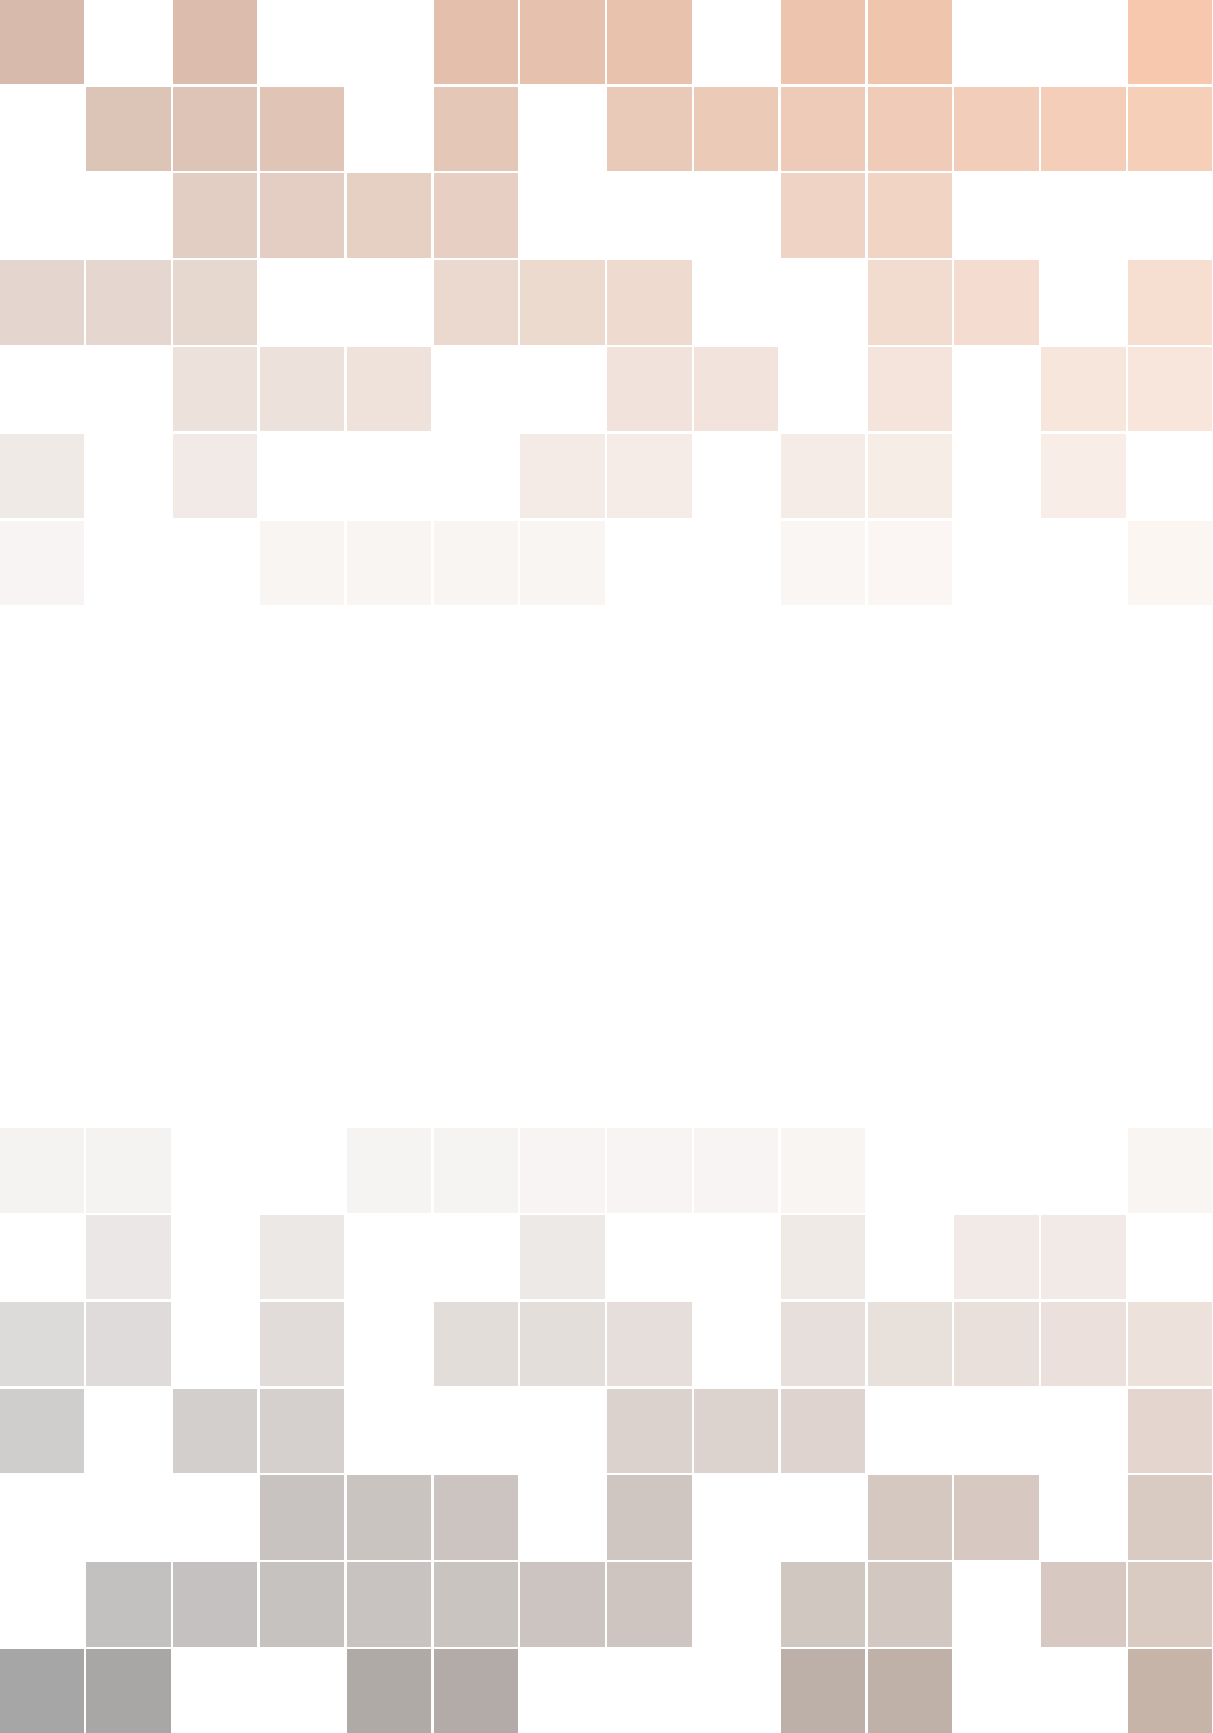
\includegraphics[width=\paperwidth]{poly/Pictures/background.pdf}};
\draw (current page.center) node [fill=ocre!30!white,fill opacity=0.6,text opacity=1,inner sep=1cm]{\Huge\centering\bfseries\sffamily\parbox[c][][t]{\paperwidth}{\centering Signal et Filtrage\\[15pt] % Book title
{\Large 2ème année IMACS }\\[20pt] % Subtitle
{\huge Alexandre Boyer, Pascal Acco, Léa Cot }}}; % Author name
\end{tikzpicture}
\vfill
\endgroup



% -------------------------------------------------------------------------
%	TABLE OF CONTENTS
%-------------------------------------------------------------------------
\usechapterimagefalse 
%\pagestyle{empty} % Disable headers and footers for the following pages
%\tableofcontents % Print the table of contents itself
%\cleardoublepage % Forces the first chapter to start on an odd page so it's on the right side of the book
\pagestyle{fancy} % Enable headers and footers again

%-------------------------------------------------------------------------
%	CHAPITRES
% -------------------------------------------------------------------------

%\tableofcontents
%\setcounter{tocdepth}{4}
%\cleardoublepage
\def\question#1{\paragraph{#1}}
\def\refWeb#1#2{\qrcode[version=1,height=1.5cm]{#2} \href{#2}{#1} 
%    \begin{pspicture}(25mm,25mm)
%      \psbarcode{#2}{}{qrcode}
%    \end{pspicture}}
}

%\chapter{LowTech}
%\begin{competences}
  Revoir de manière axiomatique, \cad{} sans rien mémoriser et en sachant retrouver à partir des axiomes, les bases de~:
  \begin{itemize}
  \item Géométrie et son utilisation pour calculer
  \item L'échelle logarithmlique et découvrir son usage pour les calculs
  \item Trigonométrie 
  \item Représentation complexe d'une onde réelle~: phaseurs
  \item Espaces Euclidiens et produits scalaires.
  \end{itemize}
  
\end{competences}

\section{Multiplier et diviser avec Thales}

\question{Calcul de racines carré}

Utilisez le théorème de Pythagore pour contruire une spirale des racines carrées et mesurer les longueurs $\sqrt{2}$, $\sqrt{3}$ et $\sqrt{5}$ sur un graphique. Sachant que
la construction peut être précise au milimètre près ($\pm 0.5mm$), quelle est le
nombre de chiffres significatifs de ces mesures.
Peut-on assurer $10\%$, $5\%$, $1\%$, ou $0.5\%$ d'erreur de calcul graphique ?
Que devient la précision lorsquel'on avance dans la spirale et comment limiter ce problème ?

\question{Précision et Thalès}
Pour une figure de Thales, on peut dire que ~:
\begin{itemize}
\item O/N --- On a forcément un petit triangle dans un grand~;
\item O/N --- Un petit triangle dans un grand peut-être une figure de Thales~;
\item O/N --- Il est nécessaire d'avoir deux côtés perpendiculaires à un troisième côté~;
\item O/N --- Il est nécessaire et suffisant d'avoir un sommet commun et les côtés opposées à ce sommet parallèles entre-eux.
\end{itemize}

Vos réponses à cette question doivent correspondre à un petit robot de \emph{Ulysse 31}.

Utilisez une figure de Thalès pour mesurer $\sqrt{2}$ avec 3 chiffres significatifs et une résolution meilleure que $1\%$.

\question{Règle de trois et Thalès}
Posez votre \og{} produit en croix\fg{} avec votre méthode habituelle pour résoudre le problème suivant~:
\og{} Monsieur Acco pèse maintenant 106 Kg après avoir augmenté sont poids  de $15\%$ pendant cet été. Combien pesait-il au début du mois de Juin ?\fg{}

Calculez à la main le résultat de la division pour avoir 3 chiffres significatifs.

Représentez maintenant ce problème sous la forme d'une figure de Thalès et mesurez le résultat.

Utilisez la bissectrice et faites une construction en escalier pour estimer le poids pour quelques années à venir et les années passées. Que pensez-vous de la rapidité et de la précision de cette méthode ?

\question{L'échelle logarithmique pour multiplier}




%\begin{minipage}{0.4\linewidth}
%  \refWeb{Corrigé \'Echantillonnage 1.1}{https://moodle.insa-toulouse.fr/mod/resource/view.php?id=104716}
%\end{minipage}




%%% Local Variables:
%%% mode: LaTeX
%%% TeX-master: "poly_td"
%%% End:




\chapter{Signaux}

\section{\'Echantillonnage de signaux fondamentaux}

\begin{minipage}{0.4\linewidth}
  \refWeb{Corrigé \'Echantillonnage 1.1}{https://moodle.insa-toulouse.fr/mod/resource/view.php?id=104716}
\end{minipage}

\def\pc{\widehat{p_c}}

\subsection{Premier ordre réel~: $e^{-t/\tau}$}

La réponse impulsionnelle d'un système continu du premier ordre est~:

$$ Y(p) = \frac{1}{1+\tau. p} X(p) \quad \underset{p.Y(p)\rightarrow \vec{\dot{y}} }{\longleftrightarrow} \quad \vec{y} + \tau \vec{\dot{y}}  = \vec{x}\quad \underset{\vec{x}=\vec{\delta_0}}{\longleftrightarrow} \quad \underbrace{h(t)}_{\vec{y}} =\frac{1}{\tau}. e^{-t/\tau}.\Gamma(t)$$


Ce système à pour pôle $\pc=-\frac{1}{\tau}$ s'écrit donc
$$ Y(p) = \frac{\pc}{p - \pc} X(p) \quad \underset{p.Y(p)\rightarrow \vec{\dot{y}} }{\longleftrightarrow} \quad \vec{\dot{y}} - \pc . \vec{y}  = \pc . \vec{x}\quad \underset{\vec{x}=\vec{\delta_0}}{\longleftrightarrow} \quad \underbrace{h(t)}_{\vec{y}} = -\pc . e^{\pc . t}.\Gamma(t)$$


\def\h#1{(#1>0)}
\def\fonc#1{1 * \h{#1} *  exp(-#1)}
\def\dirac#1{(#1<0.001)*(#1>-0.001)*1}

%\begin{tikzpicture}
\begin{tikzpicture}[outer sep=auto, amp/.style = {regular polygon, regular polygon sides=3,
    draw, fill=white, text width=1em,
    inner sep=1mm, outer sep=0mm,
    shape border rotate=-90}]
  
  \matrix (graphe)[ row sep=0cm, column sep=1cm, inner sep=0.5cm]{ 	
  \begin{scope}[] 
    \begin{axis}[	anchor = origin,  x=1cm, y=1cm,
      axis lines=center, 
      xlabel={$t[s]$},
      ylabel={$x(t) = \delta_0(t)$},
      ylabel style = {anchor=south, thick, black},
      xlabel style = {anchor=west, thick, black},
      grid=minor,
      domain=-0.5:2.5,
      ytick={0,1},
      yticklabels={0,1},
      xtick={0,1,2},
      xticklabels={0,1,2},
      enlarge y limits=0.5,
      enlarge x limits=0.1,
      help lines
      ]
      \addplot[very thick, blue,samples=512] plot (\x,{\dirac{\x}});
    \end{axis}
  \end{scope};
    & \node[dspnodeopen]  (x) {$\vec{x}$};
    & \node[dspsquare] (G) {$G(p)$} ;
    & \node[dspnodeopen]  (y) {$\vec{y}$};
    &
  \begin{scope}[] 
    \begin{axis}[anchor = origin,  x=1cm, y=1cm,
      axis lines=center, 
      xlabel={$t[s]$},
      ylabel={$y(t) = h(t)$},
      ylabel style = {anchor=south, thick, black},
      xlabel style = {anchor=west, thick, black},
      grid=minor,
      domain=-0.5:3.5,
      ytick={0,1},
      yticklabels={0,$\frac{1}{\tau}$},
      xtick={0,1,2,3,4},
      xticklabels={0,$\tau$,$2\tau$,$3\tau$, },
      enlarge y limits=0.5,
      enlarge x limits=0.1,
      help lines
      ]
      \addplot[very thick, blue, samples=512] plot (\x,{\fonc{\x}});
      \draw[dashed, thick, blue](0,1)--(1,0);
    \end{axis}
  \end{scope}

    \\
  };
  \draw[dspflow] (x) -- (G) -- (y) ;
  
\end{tikzpicture}


Ce système de pôle $\widehat{p_c}=\frac{-1}{\tau}$ est stable
s.s.i. $\tau> 0$ car~:

Stable simple $\quad \iff h(t) \underset{t\to +\infty}{\rightarrow} 0 \iff$ \og{} retour à l'équilibre après stimuli. \fg{} 

Cela corrobore le fait qu'un pôle réel est stable s.s.i
$\widehat{p_c}$ est dans le demi-plan gauche de \Laplace{}~:
$\widehat{p_c}\prec 0$.

Le terme $\Gamma(t)$ est nul pour $t<0$ (fonction de \Heaviside), on
trouve que le système est causal puisque la Réponse ImPulsionnelle
(RIp) est nulle avant la stimulation par l'impulsion~:

Système causal $\quad \iff \quad \forall t<0,\; h(t)=0 \quad \iff$ \og{} pas de réponse avant stimuli. \fg 

\question{Q1~: discrétisation de $h$} Discrétisez le signal $t\mapsto h(t)$, avec
une période d'échantillonnage temporelle $T_e$, pour obtenir le signal
$\vec{h} : k \mapsto h[k]=h(\overbrace{k\,T_e}^{t})$.

Montrez qu'il s'agit d'une suite géométrique $h[k]=a^k.\Gamma[k]$ où
vous exprimerez $a\in\R$ en fonction de $\tau$ et $T_e$.

\question{Q2~: condition de stabilité en discret} Dans l'exercice AR~(Auto Regressif)~\ref{sec:AR}, nous construirons le système discret dont la réponse impulsionnelle est $k\to h[k]$ pour obtenir un système du premier ordre discret. 

Représentez $h$ graphiquement (discret et continu si possible) pour $a=\frac{1}{2}$, puis $a=1$, puis
$2$, puis $a=-\frac{1}{2}$, puis $-1$, puis $-2$.

La condition de stabilité simple en discret reste \og{}retour à zéro
après stimuli\fg{} :
  $h[k]\underset{k\to +\infty}{\longrightarrow} 0$.

  Donnez la condition nécessaire et suffisante de stabilité du système
  $H$ en fonction de $a$ et vérifiez qu'elle correspond à celle en
  continu avec $\tau$.
  
\subsection{Oscillateur imaginaire pur : $e^{i\omega\,t}$}
Le système du premier ordre précédant peut être choisi avec un pôle
imaginaire pur $p_c= i\omega$.

$$ Y(p) = \frac{1}{p-i\omega} X(p) \quad \underset{p.Y(p)\rightarrow \vec{\dot{y}} }{\longleftrightarrow} \quad  \vec{\dot{y}} - i\omega \vec{y}  = \vec{x}\quad \underset{\vec{x}=\vec{\delta_0}}{\longleftrightarrow} \quad \underbrace{h(t)}_{\vec{y}} = e^{i\omega\,t}.\Gamma(t)$$


Le système devient un système complexe (abstrait) de réponse
impulsionnelle $h(t)=e^{i\omega\,t}.\Gamma(t)$ comportant en partie
réelle une RIp (Réponse Impulsionnelle) $\cos\!\left(\omega\,t\right)$
causal et un $\sin\!\left(\omega\,t\right)$ causal en partie imaginaire.

\question{Q1~: discrétisation de $h$} Discrétisez le signal
$t\mapsto h(t)$, avec une période d'échantillonnage temporelle
$T_e$. Montrez qu'il s'agit, là aussi, d'une suite géométrique
$h[k]=q^k.\Gamma[k]$, mais cette fois-ci avec $q\in\C$ dont vous
donnerez la relation avec $\omega$ et $T_e$.

\question{Q2~: condition de stabilité en discret} Le pôle continu
$p_c$ correspond à un système en limite de stabilité, car la RIp $h$
ne converge pas vers 0 et ne diverge pas à l'infini non plus. Ce pôle est sur l'axe imaginaire pur~: entre le demi plan gauche stable et
le demi plan droit instable divergent.

Nous verrons plus tard que $q$ est le pôle du système discret.

Déterminez le type de convergence de $\left\{h[k]\right\}$. Que devient l'axe imaginaire de limite de stabilité pour les pôles continus $p_c$ lorsque l'on passe à un système discret de pôle $q$ ?

\question{Q3~: périodicité du spectre}

Pour représenter la suite numérique complexe $\left\{h[k]\right\}$
graphiquement, on placera les points $h[k]\in\C$ dans le plan
complexe en indiquant leur indice $k$ à côté.

\begin{tikzpicture}

	\begin{axis}[
			anchor = origin,  x=1.5cm, y=1.5cm,
			ymin=-1.5, ymax=1.5,
			xmin=-1.5, xmax = 1.5,
			ytick = {0},	
			xtick={-1,1 },
			axis lines=center, 
			xlabel={$\mathbb{R}$},
			ylabel={$\mathbb{I}$},
			ylabel style = {anchor=east, thick, black},
			xlabel style = {anchor=west, thick, black},
			grid=minor,
			help lines]
 		\draw (0,0) circle (1);
		\draw [very thick, black, fill=black] ({1.3*cos(0)},{1.3*sin(0)}) circle (0.05) ;
		\draw [very thick] ({1.3*cos(20)},{1.3*sin(20)}) circle (0.05) node[right] {} ;
		\draw [very thick] ({1.3*cos(40)},{1.3*sin(40)}) circle (0.05) node[right] {} ;
		\draw [very thick] ({1.3*cos(60)},{1.3*sin(60)}) circle (0.05) node[right] {} ;
		\draw [thick,->] ({1.3*cos(3},{1.3*sin(3)}) arc (3:17:1.3)  node[right] {} ;
		\draw [thick,->] ({1.3*cos(23)},{1.3*sin(23)}) arc (23:37:1.3) node[right] {} ;
		\draw [thick,->] ({1.3*cos(43)},{1.3*sin(43)}) arc (43:57:1.3) node[right] {} ;
		\draw [thick,->,dashed] ({1.3*cos(63)},{1.3*sin(63)}) arc (63:77:1.3) node[right] {} ;
		\node [black ,  thick] (q0) at (1.4,0.2) {$q^0$};
		\node [black ,  thick] (q1) at (1.4,0.6) {$q^1$};
		\node [black ,  thick] (q2) at (1.2,0.9) {$q^2$};
		\node [black ,  thick] (q3) at (0.9,1.2) {$q^3$};
\end{axis}

\end{tikzpicture}

Représentez graphiquement $\vec{h}$ pour $q=e^{i\,\frac{\pi}{2}}$,
vous remarquerez que ce signal est $4$ périodique~: on le notera
$h_4$.

Représentez alors la suite numérique $h_4$ par un tuple de
4 valeurs complexes~:

$\ldp\overbrace{1}^{k=0},q, q^2, q^3\rdp = \ldp q^3, \overbrace{1}^{k=0},q, q^2 \rdp=\dots$ où les doubles parenthèses indiquent que la suite est périodique.

Faites de même avec $q=e^{i\,\frac{5\pi}{2}}$ et
$q=e^{i\,\frac{-3\pi}{2}}$. Cela devrait vous aider à trouver,
pour une pulsation d'échantillonnage
$\omega_e=2\pi\,F_e=\frac{2\pi}{T_e}$ donnée, \textbf{TOUTES}
les pulsations $\omega$ qui permetttent d'avoir ce signal
discret 4 périodique $h_4$.

\begin{remarque}
  On en déduit que toute les ondes continues pures de
  pulsation $\omega + n.\omega_e$, et donc de fréquence
  $f + n.F_e$, donnent exactement le même signal discret~!

  Lorsque l'on observe un signal fini de N échantillons, la
  transformée de \Fourier{} d'un Signal Discret (TFSD) étend ce signal
  par des zéros pour obtenir la suite infinie

  
  $( \dots,0,0, \overbrace{s[0]}^{}, \dots s[N-1],0,0,\dots)$ à
  support borné.

  
  Il suffit de décomposer/calculer la TFSD uniquement pour les
  fréquences $f \in \left[0 , F_e\right[$. En effet, la composante
  discrète à la fréquence $f$ est $e^{i\,2\pi\,f\,\frac{k}{F_e}}$ et
  un calcul pour une fréquence $f + n.F_e$ donnerait le même résultat
  que pour $f$ puisque on aurait exactement le même signal discret.

  Un signal discret est ainsi transformé par \textbf{la TFSD en
    fonction continue de $f$ qui est $F_e$ périodique} et seule les
  fréquences $0\le f<F_e$ sont utiles.
  
  Seul l'incrément angulaire $\Delta$ de
  $q=e^{i.\overbrace{2\pi\frac{f}{F_e}}^{\Delta}}$
  identifie une onde pure discrète. On
  préfère alors  utiliser la \textbf{fréquence normalisée}
  $\frac{f}{F_e}$, notée $\tilde{f}$.
  
\end{remarque}

\question{Q4 : signaux temporel  périodiques et spectre discrets}

On cherche maintenant toute les fréquences pouvant donner un signal
temporel de période 8.  Représentez graphiquement le signal de
fréquence normalisée $\tilde{f_0}=\frac{1}{8}$ pour
$q=e^{i\,2\pi\frac{1}{8}}$ et vérifiez la question précédente avec les
fréquences $\tilde{f}=\frac{9}{8}$ et $\tilde{f}=\frac{-7}{8}$ par
périodicité du spectre en fréquence.


Donnez la séquence $\ldp \overbrace{1}^{},\dots, q^7 \rdp$ pour
vérifier que ce signal discret est bien 8 périodique.

Quelles sont les périodes des signaux à $2\tilde{f_0}$, $3\tilde{f_0}$, $4\tilde{f_0}$ ? Sont-ils tous 8-périodiques ?

Généralisez, en gardant $k$ l'indice temporel de $t=k.T_e$ et en prenant $n$ pour indice des fréquences de $f=n.\tilde{f_0}=n\frac{F_e}{N}$. On montrera que les ondes pures $e^{i.2\pi.\overbrace{n\,f_0}^{f}.\overbrace{k\,T_e}^{t}}$ sont toutes N périodiques dans le temps. 
\begin{remarque}

  Contrairement à la TFSD qui étend un signal à l'infini avec des zéros, la TFD/FFT (Transformée de \Fourier{} Discrète, et son algorithme de calcul rapide Fast Fourier Transform) considère que le signal est N périodique de la forme $\ldp \overbrace{s[0]}^{}, \dots s[N-1] \rdp$.
  
  On montre facilement qu'une fonction N périodique ne peut être
  décomposée que par des fonctions N-périodiques. Seules les ondes de
  fréquence multiples $n.f_0= n.\frac{F_e}{N}$ sont N périodiques et
  donc utiles pour décomposer le signal.

Un signal complexe de N points en temporel est donc transformé par \textbf{la TFD en un signal discret de N points complexes données aux fréquences $f \in \left\{n.f_0 | 0 \le n<N\right\}$.}
La TFD est donc un \textbf{signal discret en fréquence} échantillonné à la \textbf{résolution $f_0=\frac{F_e}{N}$} appellée \textbf{résolution fréquentielle}.

\end{remarque}


Pour dessiner l'échelle de fréquence d'une TFD, dessinez un axe fréquentiel en indiquant les fréquences normalisées allant de $\frac{-3}{8}$ à $\frac{13}{8}$.

Complétez cette échelle en indiquant les fréquences équivalentes les
plus petites en valeur absolue : par exemple remplacer $\frac{9}{8}$
par $\frac{1}{8}$ par périodicité du spectre de la question~3~; mais
aussi, remplacer $\frac{7}{8}$ par $-\frac{1}{8}$.

En déduire que la fréquence la plus rapide en discret n'est pas infinie~! Cette fréquence est la fréquence de Nyquist.


\question{Q5 : Dualité, conjugué et antipodal}

Représentez la suite de fréquence $\tilde{f}=\frac{-1}{8}$. Vous devez
constater que l'on obtient le \textbf{signal antipodal} (signal joué à
l'envers~:$k\to h[-k]$) de $h_8$.

De même vous remarquez que ce signal, noté $h_{-8}$, pour la fréquence $\tilde{f}=\frac{-1}{8}$ est aussi le conjugué de $h_8$ à la fréquence $\tilde{f}=\frac{1}{8}$.



%%% Local Variables:
%%% mode: LaTeX
%%% TeX-master: "poly_td"
%%% End:


   
% \chapter{Systèmes}

% \begin{minipage}{0.4\linewidth}
%   \refWeb{Corrigé MA 1.1}{https://moodle.insa-toulouse.fr/mod/resource/view.php?id=89521}
% \end{minipage}
% \begin{minipage}{0.4\linewidth}
%     \refWeb{Corrigé AR 1.2}{https://moodle.insa-toulouse.fr/mod/resource/view.php?id=89522}
% \end{minipage}
% \begin{minipage}{0.4\linewidth}
%   \refWeb{Corrigé ARMA 1.3}{https://moodle.insa-toulouse.fr/mod/resource/view.php?id=89523}
% \end{minipage}

% 
 \section{MA : systèmes Mooving Average à moyenne glissante.}


\graphe{0.6\textwidth}{../../poly/tikz/ma_ab.png} 

Les cercles sont des multiplieurs, l'opérateur T est le retard unitaire, le cercle avec un + est un additionneur.



\question{Q1~: Block $\rightarrow$ Récurrence ou Équation différentielle} 
\refWeb{Vidéo MA1 : Block -> récurrence}{https://youtu.be/QRiAfbWLMw8?t=107}


Passez du schéma block à l'équation aux différences (récurrence) que vous mettrez sous forme :  
\begin{itemize}
\item $y[k+1]=\ldots$  
\item $y[k]=\ldots$  
\end{itemize}
Simplifiez les expressions et dites de quel ordre est ce système.  



\question{Q2~: Récurrence $\rightarrow$ Fonction de transfer $G(z)$} 
\refWeb{Vidéo MA1 : Récurrence -> G(z)}{https://youtu.be/QRiAfbWLMw8?t=479}

En se rappelant que $z^{-1}$ est le système/signal associé à
l'opérateur retard $T$, donnez la fonction de transfert en Z en
partant de chaque récurrence :
\begin{itemize}
\item $y[k]=\ldots \implies Y(z) = \overbrace{\ldots}^{G(z)} \;.\; X(z) $  
\item $y[k+1]=\ldots \implies z.Y(z) =  \overbrace{\ldots}^{G(z)} \;.\; z.X(z)$
\end{itemize}



\question{Q3~: Caractérisation et propriétés (LTI, causal,  \dots)}

Identifiez les trois types d'opérateurs utilisés et dites pour chacun
si ce sont des systèmes LTI (Linéaire à Temps Invariant), des systèmes
causaux.  Conclure si le système entier est lui-même LTI, causal.

Le système est-il~:
\begin{itemize}
\item auto-regressif ?
\item récurrent ?
\item à moyenne glissante (mooving
  average) ?
\item bouclé ?
\end{itemize}





\question{Q4~: G(z) $\rightarrow$ Réponse Impulsionnelle (RIp) }
\refWeb{Vidéo MA2 : Transformée inverse de H(z)}{https://youtu.be/sKBlBBVbRWw?t=252}

Utilisez la fonction de transfert $Y(z) = G(z) . X(z)$ pour trouver la
transformée de la réponse impulsionnelle
$H(z) = G(z) . \tZde{\vec{\delta_0}}$.

Utilisez la transformée inverse pour retrouver la réponse
impulsionnelle temporelle $\vec{h} = \tZiDe{H(z)}$

\begin{remarque}
  Rappelez-vous comment un système/opérateur $X(z)$ (à base des
  opérateurs cités en Q3) est associé à un signal unique
  $\vec{x}: k\mapsto x[k]$ temporel.

  Indice~: signal RIp $\to$ système. Gros indice~:
  $\vec{x}=X (z)\!\left\{\vec{\delta_0}\right\}$

  Utilisez la phrase \og{}Une impulsion unité en entrée d'un gain de 1
  produit une impulsion unité\fg{} pour en déduire $\tZde{\vec{\delta_0}}$~: la transformée en
  $z$ de l'impulsion unité $\delta_0$.

  Traduisez la défintion de la fonction de transfert
  $Y(z) = G(z) . X(z)$ en un schéma block qui explique comment
  produire un signal de sortie temporel $\vec{y}: k \mapsto y[k]$ à
  partir d'une impulsion unité. Indice~:
  $\vec{y}=G(z)\left\{\overbrace{ X(z)\!\left\{ \vec{\delta_0} \right\}}^{\vec{x}} \right\}$

  L'association $X (z)\!\left\{\vec{\delta_0}\right\}=\vec{x}$ définit
  la transofrmée $X(z) = \tZde{\vec{x}}$. La transformée inverse $\tZiDe{H(z)}=\vec{h}$
  se trouve, sans calcul analytique à faire !, par l'association inverse.

  Indice~: Système  $\to$ RIp. Gros indice $\vec{h} = H(z)\!\left\{\vec{\delta_0}\right\}$

\end{remarque}

À partir de la réponse impulsionnelle concluez si le système est
FIR (Finite Impluse Response) ou IIR (Infinite Impulse response) ?


\question{Q5~: Schéma Block MA $\rightarrow$ RIp} \refWeb{Vidéo MA2 : RIp et Causalité}{https://youtu.be/sKBlBBVbRWw?t=523}

Donnez la réponse impulsionnelle des systèmes~: \og{} gain de a\fg{} ; \og{} gain de b\fg{} ; d'un retard unitaire $T$.

Rappelez la relation temporelle entre la sortie $\vec{y}$ d'un système de RIp $\vec{h}$ pour une entrée $\vec{x}$.

Dans le schéma block, remplacez l'entrée $x[k]$ par l'impulsion
$\vec{\delta_0}$ et propagez le signal dans le schéma block jusqu'à la
sortie (par exemple la sortie du gain $b$ donnerait
$\vec{\delta_0} \star (b.\vec{\delta_0}) = b.\vec{\delta_0}$.

Que devient la relation $Y(z) = G(z) . X(z)$ en schéma block puis en
temporel $\vec{y} = \dots$



\question{  Q6 }
Retrouvez la propriété de causalité de la Q1 mais à partir de la RIp $h$. 


\question{  Q7 }

Quelle propriétée doit vérifier la RIp pour que le système soit stable
? Est-ce une condition nécessaire et suffisante ?

Concluez si ce système est BIBO stable à partir de sa RIp.

BONUS : démontrez que $\Sigma h$ ACV $\implies$ H stable

\question{  Q8 }

Donnez un schéma block en transformée en Z sous forme simplifiée Directe I (chaîne de retards puis combinaison linéaire). Retrouvez de quel ordre est ce système.

\question{  Q9 }
On appelle BIBO la propriété de stabilité : "Bounded Input Bounded Output"

A-t-on :

\begin{itemize}
\item  $MA \implies FIR$ ?  
\item $FIR \implies BIBO$ ? Ou $BIBO \implies FIR$ ? Ou $BIBO \iff FIR$ ?  
\item $MA \implies FIR \implies BIBO$ ?  
\item $BIBO \iff FIR \implies MA$ ?  
\end{itemize}

%%% Local Variables:
%%% mode: latex
%%% TeX-master: "poly_td"
%%% End:

% \section{AR : Système Auto-Régressif (AR)} 
\label{sec:AR}
La réponse impulsionnelle d'un système continu du premier ordre est~:

$$ Y(p) = \frac{1}{1+\tau. p} X(p) \quad \underset{\vec{x}=X(p)\left\{\vec{\delta_0}\right\}}{\longleftrightarrow} \quad \tau \vec{y} + \vec{\dot{y}} = \vec{x}\quad \underset{\vec{x}=\vec{\delta_0}}{\longleftrightarrow} \quad h(t) = e^{-t/\tau}.\Gamma(t)$$

Ce système de pôle $\widehat{p_c}=\frac{-1}{\tau}$ est stable s.s.i.
$h(t) \underset{t\to \infty}{\rightarrow} 0$ donc s.s.i. $\tau\succ 0$
(dans le cas général où $\tau \in \C$, $\tau\succ 0$ veut dire que la
partie réelle de $\tau$ est positive). Cela permet de retrouver le
fait qu'un pôle est stable s.s.i $\widehat{p_c}$ est dans le demi-plan gauche de
Laplace~: $\widehat{p_c}\prec 0$.


Nous voulons créer un système discret capable de
générer la même réponse impulsionnelle de durée infinie (asymptotique)~:

$$Y(z) = \frac{\dots}{\dots +\dots z} X(z) \quad \underset{\vec{x}=X(z)\left\{\vec{\delta_0}\right\}}{\longleftrightarrow} \quad  \dots \vec{y[\bullet]} + \dots. \vec{y[\bullet-1]} = \dots . \vec{x}\quad \underset{\vec{x}=\vec{\delta_0}}{\longleftrightarrow} \quad h[k] = h\left(k.T_e\right) = a^k.\Gamma[k]$$

Les pôles $\widehat{p_d}$ de cette fonction de transfert discrète pourraient, de même, donner un lieu géométrique des pôles discrets stables comme le demi-plan gauche du continu.



\question{Q1~: $h \quad \rightarrow  $ récurrence $\quad \rightarrow G(z) $}

\refWeb{Vidéo AR1 : Récurrence}{https://youtu.be/TjNE5sKsKRM?t=19}

Donnez l'expression sous forme de récurrence d'une suite géométrique
de raison $a$ et essayez d'identifier cette récurrence à celle d'une
récurrence d'un système discret d'entrée $x$ et de sortie $y$.


\begin{remarque}
  Une récurrence avec condition initiale est un \emph{système à
    mémoire} (avec dans notre cas $y[0]=1$ et $y[k<0]=0$) mais
\emph{sans entrée} (le système à entrée nulle est dit autonome)~:
 
 $y[k]=a.y[k-1] \quad \forall k>0$ avec condition initiale $y[0]=1$

 De manière équivalente, on construit un \emph{système sans mémoire}
 (à mémoire nulle $y[k\leq 0]=0$) mais \emph{avec entrée}
 $\vec{x}=\vec{\delta_0}$ pour établir la \emph{condition initiale
   (CI)} $y[0]=1$ :
  
 $y[k]=a.y[k-1] + x[k] \quad \forall k\in\mathbb{Z}$ avec C.I. nulles
 $y[k<0]=0$.
 
 
\end{remarque}


Si vous n'y arrivez-pas facilement, faites d'abord la question suivante.

Sinon, donnez la fonction de transfert $G_1(z)$ de cette récurrence et
faites le lien avec celle de la question suivante.


\question{Q2~[optionnelle]~: Schéma Bloc $\quad\rightarrow\quad$ récurrence $\quad\rightarrow\quad h[\bullet-1]$ } 

\graphe{0.8\textwidth}{../../poly/tikz/ar_o1.png}


Traduisez ce schéma bloc en récurrence, puis en fonction de transfert (notée $G_T(z)$).

Calculez-en la réponse impulsionnelle $h$ à partir de l'équation de récurrence.


\begin{remarque}
  
  \refWeb{Vidéo G(z) → RIp}{https://youtu.be/_Mrx9QQ-z5o?t=1366}
  Apprenez à faire une division par les puissances décroissante. Puis
  vérifiez les premiers termes de $h$ en faisant la division par les
  puissances décroissantes de~:
\begin{itemize}
\item $\frac{z}{z^2-az}$ (récurrence en $y[k+2]=\dots$)~; ou de
\item $\frac{1}{z-a}$ (récurrence en $y[k+1]=\dots$)~; ou encore de
\item $\frac{\zmu}{1-a\zmu}$ (récurrence en $y[k]=\dots$).
\end{itemize}
\end{remarque}
On doit obtenir notre suite géométrique avec un peu de retard ;-) ...


La fonction de transfert $G_1(z)$ de la Q1 donne la suite géométrique $h$ en RIp.

La fonction de transfert $G_T(z)$ donne cette suite avec un retard unitaire.

Donnez donc la relation $G_?(z) = z^{?}.G_?(z)$ qui exprime qu'un système est en avance sur l'autre.


\question{Q3~[Optionnelle]~: $h \quad \rightarrow \quad H(z) = G(z) $ }


La fonction de transfert $G_1(z)$ de notre système à pour réponse
impulsionnelle $h$ donc
$$H(z) = G_1(z).\underbrace{1}_{Z\{\delta_0\}}$$

Il en résulte que $G_1(z)=H(z)$ et donc $G_1(z)=\tZde{\vec{h}}$. On
peut donc trouver la fonction de transfert en calculant la transformée
de la RIp $\vec{h}$.

\begin{remarque}
  Tout signal se décompose dans le temps sous forme de somme d'impulsions unité~:

  $\vec{h}= h[0].\vec{\delta_0} + h[1].\vec{\delta_1} + h[2].\vec{\delta_2} + \dots$.

La transformée en Z de cette combinaison linéaire de retards d'impulsions unité est triviale~:  

$H(z)= h[0].\underbrace{1}_{\tZde{\vec{\delta_0}}} + h[1].\underbrace{\zmu}_{\tZde{\vec{\delta_1}}} + h[2].\underbrace{z^{-2}}_{\tZde{\vec{\delta_2}}} + \dots$.

Ce qui donne la formule analytique de la transformée en Z~:
$$\tZde{\vec{h}} = H(z) = \sum\limits_{j=-\infty}^{\infty} h[j] . z^{-j}$$
Dans la plupart des ouvrages, $z$ est un nombre complexe et le domaine
de convergence de cette série entière doit être donné~: valeur de
$z\in\C$ où la somme converge.

Dans ce cours, la variable $z$ est l'opérateur avance unitaire et on décrit simplement le système $H(z)$, qui produit $h$ en RIp, en  utilisant la décomposition de $\vec{h}$ dans le temps.

\end{remarque}

Dans notre cas, la suite géométrique temporelle $\left(h[k]\right)$ devient une suite géométrique de l'opérateur $z$.

Retrouvez la formule de la somme d'une série géométrique pour
retrouver $H(z)$ sous forme d'une fraction rationnelle en $z^{-1}$.

\begin{remarque}
  La somme partielle d'une suite géométrique se trouve facilement par effet télescopique~:

\begin{equation*}
  \begin{array}{cccccccc}
    S_n       &=&   q^0     &+q^1   & +\dots &  + q^{n} &  \\
    -q.S_n     &=&         &-q^1 & +\dots & - q^{n} &- q^{n+1}  \\\hline
    (1-q).S_n &=&   q^0  &       &         &       & -q^{n+1}
  \end{array}
\end{equation*}
Lorsque la raison $q$ de la suite est inférieure en module à 1, la
limite de $S_n$, lorsque $n\to \infty$, se simplifie car $q^{n+1}\to 0$.
\end{remarque}


Vous obtenez ainsi la fonction de transfert $H(z)=G_1(z)$ sous forme de fraction rationnelle. 
\begin{remarque}
  Apprenez à faire une division par les puissances croissantes et
  faites une division par les puissances croissante de $z^{-1}$ de
  $H(z)$ pour retrouver $H(z)$ sous forme d'une suite géométrique...


  \refWeb{Vidéo G(z) → RIp}{https://youtu.be/_Mrx9QQ-z5o?t=1366}  
\end{remarque}


\question{Q4~: conditions de stabilité avec $G(z)$}


Déterminez l'ordre, le pôle $\widehat{p_c}$ et les zéros de
$G(p)=\frac{1}{1+\tau.p}$ en fonction de $\tau$. 


Déterminez de même l'ordre, le pôle $\widehat{p_d}$ et les zéros de $G_1(z)$
en fonction de $a$ puis de $\tau$ (et de $T_e$ bien
sur). \textbf{Attention ! Il faut exprimer en fonction de $z$ et non
  $z^{-1}$}

On montre, en continu, qu'un pôle est stable $\iff h(t) \to 0 \iff \tau\succ 0 \iff \text{pôle continu} \prec 0$ et donc le fameux ``demi-plan gauche stable ''.

On a montré, en discret, que stable $\iff h[k] \to 0 \iff |a|<1$. Quelle est alors la région du plan complexe où les pôles discrets sont stables. 

Pour mémoriser ce résultat fondamental, dessinez à gauche le plan
complexe et la région des pôles stable en continu, en donnant la
fonction de transfert $g(p)$ et indiquant la valeur du pôle continu
$\widehat{p_c}$.  Puis indiquez à droite de ce schéma la fonction de transfert
$G_1(z)$, l'expression de son pôle discret $\widehat{p_d}$ et la région stable
des pôles en discret.  Quelle est la condition de stabilité en discret
en fonction des zéros et des pôles ?

\begin{remarque}
La relation $\widehat{p_d} = e^{-\widehat{p_c}.T_e}$ permet de faire le lien entre un
pôle oscillant amortis en continus et son équivalent (même RIp mais
échantillonnée) en discret. Cela est utile pour savoir où placer les
pôles lors du calcul d'une commande par placement de pôles.
\end{remarque}
\question{ Q5 }
Ce système est-il MA (moyenne pondérée glissante) ? AR (auto-régressif) ? Récursif ? Bouclé ?


\question{ Q7 }
Donnez un schéma bloc en transformée en Z sous forme Directe I (chaîne de retards et combinaison linéaire). 

Retrouvez de quel ordre est ce système.

\question{ Q8 }
On appelle BIBO la propriété de stabilité : "Bounded Input Bounded Output"

A-t-on :  
\begin{itemize}
\item $IIR \implies AR$ ?
\item $IIR \implies \overline{BIBO}$ ? Ou bien $ \overline{BIBO} \implies IIR$ ? Ou bien $\overline{BIBO} \iff IIR$ ?
\item $AR \iff IIR \implies \overline{BIBO}$ ?
\item $\overline{BIBO} \implies IIR \implies AR$ ?
\end{itemize}
%%% Local Variables:
%%% mode: latex
%%% TeX-master: "poly_td"
%%% End:

% \section{ARMA~: Auto Regressive Mooving Average}


\begin{tikzpicture}[outer sep=auto]

	\matrix (graphe)[ row sep=1cm, column sep=1cm, inner sep=0.5cm]{ 	
	\node[dspnodeopen]  (x) {$x[k+1]$};																&
	\node[dspnodefull]  (tx) {};													 							&
	\node[dspsquare]  (Tx) {T};																				&
																																	&
	\node[dspsquare ]  (Ty) {T};																			&
	\node[dspmultiplier, dsp/label=  above]  (a) {$a$};								&
	\node (coin)	 {}		;																							&
																																	&
																																	\\
																																	&
																																 	&
																																	&
	 \node[dspadder ]  (S) {};																				    &
																																    &
																																    &
	\node[dspnodefull]  (ty) {};																				&
	\node[dspnodeopen,  dsp/label=above]  (y) {$y[k+1
]$};  							&\\
	};
	\draw[dspflow] (x) -- (tx) ;
	\draw[dspflow]  (tx)  -- (Tx);
	 \draw[dspflow, rounded corners=1cm] (Tx) -|  (S);
	\draw[dspflow, rounded corners=1cm] (tx)  |- (S);
	\draw[dspflow, rounded corners=1cm]  (ty) |- (a);
	 \draw[dspflow] (a) -- (Ty);
	\draw[dspflow, rounded corners=1cm] (Ty)  -| (S);
	\draw[dspflow] (S)  -- (ty);
	\draw[dspflow] (ty) -- (y);

      \end{tikzpicture}
      
\question{ Q1~: Manipulation de schéma bloc}
Repérez le(s) bouclages(s) (AR) et les moyennes glissantes (MA) et décomposez le schéma bloc en séparant clairement MA puis AR.

$\vec{x} \overset{MA}{\longrightarrow} \vec{w} \overset{AR}{\longrightarrow} \vec{y}$


\refWeb{Vidéo Schéma bloc MA-AR (s'arrêter avant AR-MA)}{https://youtu.be/TjNE5sKsKRM?si=83cs8c0a03OJ7mqv&t=805}

\question{Q2~: Bloc → Fonction de transfert}

On note l'opérateur retard $q=z^{-1}$. Donnez, en les exprimant d'abord avec des retards $q$ puis avec des avances $z$, les fonctions de transfert~:
\begin{itemize}
\item $MA(z)=\frac{W(z)}{X(z)}$, 
\item $AR(z)=\frac{Y(z)}{W(z)}$,
\item la fonction de transfert totale $G(z)=\frac{Y(z)}{X(z)} =  \underbrace{\frac{Y(z)}{W(z)}}_{AR(z)} . \underbrace{\frac{W(z)}{X(z)}}_{MA(z)} = \underbrace{\frac{W(z)}{X(z)}}_{MA(z)} . \underbrace{\frac{Y(z)}{W(z)}}_{AR(z)}$.   
\end{itemize}


\question{ Q3~:Stabilité - Pôles et zéros}
Identifiez les pôles et les zéros du système et concluez sur la stabilité en fonction de $a$.

\question{ Q4~: F. Transfert → Équation aux Différences}
Donnez, à partir de $G(1/q)$, la récurrence  du système sous forme

$y[k+1]= \ldots y[k] + \ldots x[\ldots] \ldots x[\ldots]$

et vérifiez qu'elle correspond au schéma bloc.

\question{ Q5~: F.T. → Réponse Impulsionnelle}
Trouvez la réponse impulsionnelle (on prendra $a=\frac{1}{2}$) en décomposant $G(z)$ en $MA(z)$ (numérateur FIR) puis $AR(z)$ (dénominateur IIR) :
\begin{itemize}
\item exprimez la réponse impulsionnelle du MA sous forme de deux
  impulsions
\item exprimez la réponse impulsionnelle de l'AR en réutilisant
  les résultats de l'exercice MA (1er ordre)
\item par linéarité du
  système, trouvez $h$ comme la somme des réponses AR à une somme
  finie d'impulsions issue du MA(FIR)
\end{itemize}

\begin{remarque}
N'oubliez pas que les systèmes sont causaux et que \emph{si l'on
  retarde un signal causal, il faut aussi retarder l'échelon de
  Heaviside} : utiliser par exemple $a^{k-1}u[k-1]$ pour annuler la
réponse pour $k<1$
\end{remarque}

\question{ Q6~: Idem par division en puissances croissantes}
Vérifiez le résultat en faisant une division par les puissances croissantes de $q = z^{-1}$ de la fonction de transfert totale $G(z)$ prise avec une entrée impulsionnelle. 

Vous vérifierez ainsi sur les quelques premiers termes que la réponse de la Q5 fonctionne.

\question{ Q7~: RIp → causalité et stabilité}
À partir de $h$ dites pourquoi le système est stable et causal. Vérifiez la cohérence avec la Q3.

\question{ Q8~: Manipulation de blocs → forme canonique Directe II }

\refWeb{Vidéo ARMA : Forme Directe II}{https://youtu.be/TjNE5sKsKRM?t=844}

Nous avons $G(z) = MA(z).AR(z) = AR(z).MA(z)$.  
Redessinez le schéma bloc en séparant d'\textbf{abord le AR} puis le MA.  


$\vec{x} \overset{AR}{\longrightarrow} \vec{w} \overset{MA}{\longrightarrow} \vec{y}$


En permutant le multiplieur avec le retard, regroupez les deux blocs mémoires pour n'en faire qu'un, dont l'entrée sera $w[k+1]$ et la sortie $w[k]$. 


Vous obtenez ainsi la \emph{forme Directe II} canonique (et optimale en termes de mémoire).

\question{Q8 (Optionnelle)~: Équa. Diff. → Espace d'état}

Donnez l'ordre de ce système et la récurrence sous forme de
représentation d'état discrète avec pour vecteur d'état

${}^T\!W_k = {}^T\![w[k-N], \;w[k-(N-1)], \;\ldots, w[k]]$ de taille adéquate :  

\begin{equation*}
  \left\{
    \begin{array}{cccc}
      W_{k+1} &=& A . W_k &+ B. x[k] \\
      y[k] &=& C . W_k &+  D. x[k]
    \end{array}\right.
\end{equation*}


\question{Q9~: F.T. → Réponse harmonique (Bode)}

Nous prenons maintenant $a=1$. Donnez la réponse harmonique de ce
système. Pour cela passez de $AR(z)=AR(\frac{1}{q})$ à une
représentation en fréquence $AR(i\omega)$, puis pour $MA(z)$ et enfin
pour $G(z)$.
 

Dans chaque expression faites apparaître uniquement des termes en $e^{i\,2\pi\,\tilde{f}}$ où on note $\tilde{\omega}=\frac{\omega}{\omega_e}=\tilde{f}=\frac{f}{Fe}$ la fréquence normalisée.


Dans chaque expression vérifiez~:  
\begin{itemize}
 \item que la réponse harmonique en $f$ est $f_e$ périodique (et donc 1 périodique en $\tilde{f}$)
 \item que la réponse est celle d'un système réel, c'est-à-dire, spectre de Hilbert : $G(-\tilde{f})=\overline{G(\tilde{f})}$
 \end{itemize}

 
 \begin{remarque}
 Astuce de \emph{l'arc moitié} :
 Simplifiez bien les paires d'exponentielles ! C'est \emph{très fréquent en discret}~:  

 $1 + e^{i.b} = e^{-i.b/2} (e^{i.b/2} + e^{-i.b/2}) = e^{-i.b/2}.2.\cos(b)$ et  

 $1 - e^{i.b} = e^{-i.b/2} (e^{i.b/2} - e^{-i.b/2}) = e^{-i.b/2}.2i.\cos(b)$ et  

 $e^{i.a} + e^{i.b} = e^{i.\frac{a+b}{2}} (e^{i.\frac{a-b}{2}} + e^{-i.\frac{a-b}{2}}) = e^{i.\frac{a+b}{2}}.2.\cos\left(\frac{a-b}{2}\right)$  

 $e^{i.a} - e^{i.b} = e^{i.\frac{a+b}{2}} (e^{i.\frac{a-b}{2}} - e^{-i.\frac{a-b}{2}}) = e^{i.\frac{a+b}{2}}.2i.\sin\left(\frac{a-b}{2}\right)$
 
 Comme le dit M. Lebotlan~: "Seul un Lycéen mémoriserait ces formules. 
  Alors qu'en maternelle ils savaient déjà factoriser par la moitié et puis faire comme Euler et puis c'est tout !"
\end{remarque}
Pour faire le tracé de la réponse harmonique, faites des équivalents pour avoir les asymptotes :
\begin{itemize}
\item  un équivalent pour $\tilde{f} \to 0$ doit donner une constante~;
\item un équivalent pour $\tilde{f} \to \infty$ est impossible, car la réponse est périodique ! 
\item La fréquence discrète la plus haute que l'on puisse imaginer est $\frac{F_e}{2}$ : faites donc un équivalent $\tilde{f} \to \frac{1}{2}$

\end{itemize}
  
   
%%% Local Variables:
%%% mode: latex
%%% TeX-master: "poly_td"
%%% End:


\end{document}
